\documentclass[hidelinks,12pt,a4paper]{article}
\usepackage[italian]{babel}
\usepackage[utf8]{inputenc}
\usepackage{fourier} 

% Images
\usepackage{graphicx}
\usepackage{caption}
\usepackage{subcaption}
\usepackage{float}
\graphicspath{ {../Images} }

% Stop hyphenation
\usepackage[none]{hyphenat}

% Dotted frame.
\usepackage{tikz}

% License
\usepackage[
type={CC},
modifier={by-nc-sa},
version={4.0},
]{doclicense}

\begin{document}
	
	\title{\textbf{\centering{Laboratorio creativo per bambini.}\\Collega le immagini alla descrizione.}}
	\author{Alice Balestieri}
	\date{}
	
	\maketitle
	\newpage
	
%-------- Starting images & descriptions section --------
	\begin{figure}[h]
			\centering
			\begin{tikzpicture}
				\node[draw,dashed]
				{
					\fboxrule=4pt			
					\fcolorbox{white}{white}{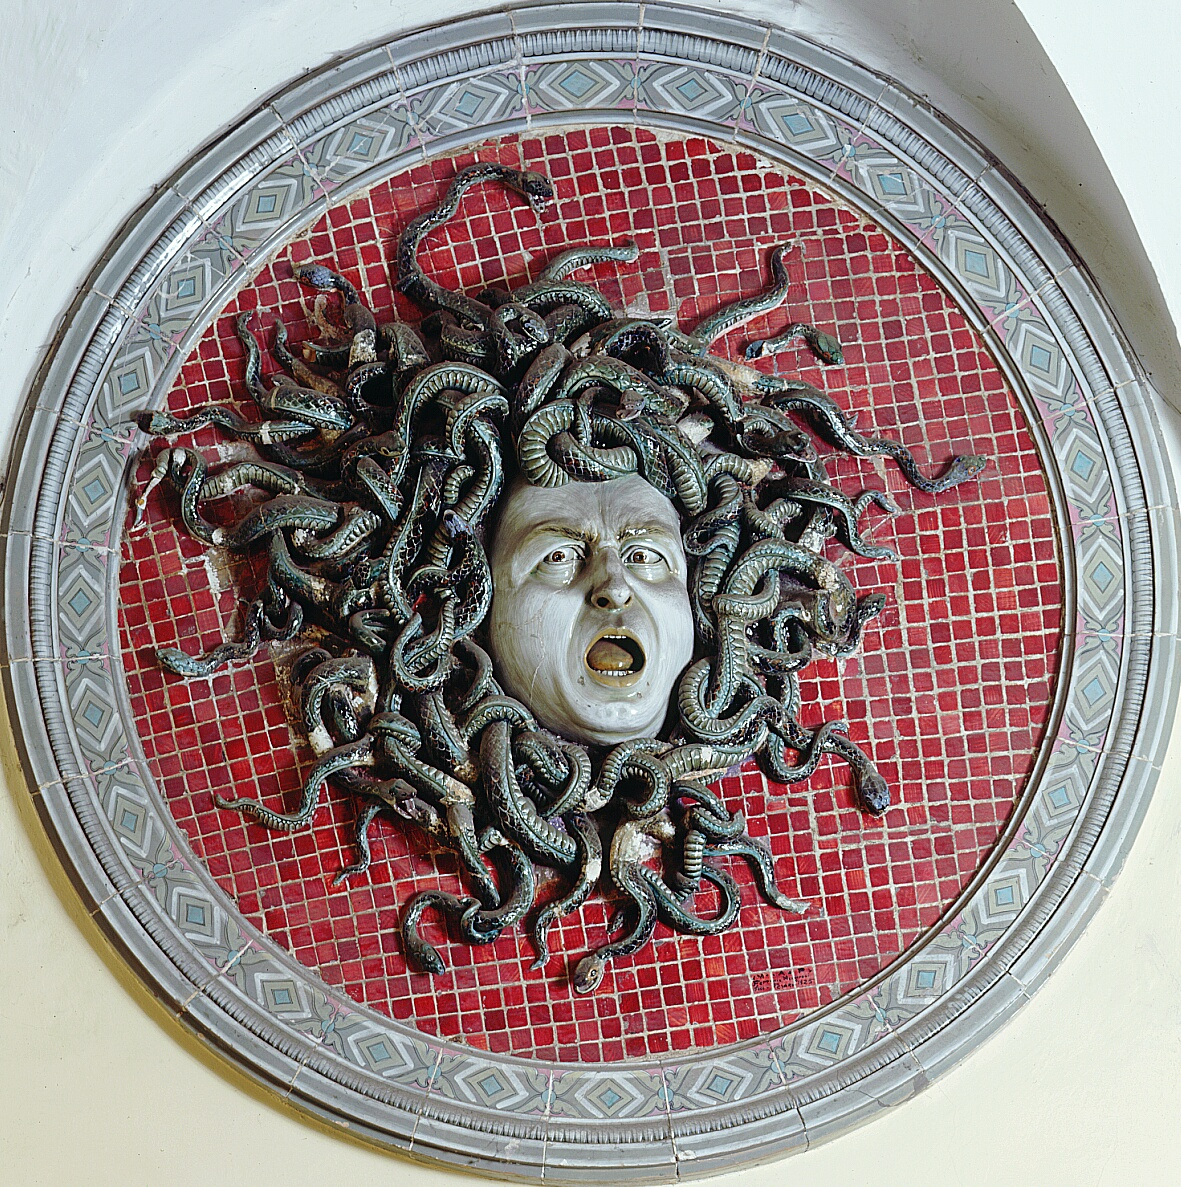
\includegraphics[scale=1.5]{Mengaroni_Ferruccio-Medusa.jpg}}
				};
			\end{tikzpicture}
	\end{figure}

	\addvspace{10mm}

	\begin{minipage}{\linewidth}
		\centering
		\begin{tikzpicture}
				\node[draw,dashed]
				{
					\fboxrule=4pt
					\fcolorbox{white}{white}{
						\fbox{
							\begin{minipage}{50mm}
								La testa della Medusa, circondata da molte serpi sinuose, raffigura il volto di Ferruccio Mengaroni; il fondo del tondo ? a tessere rosse. Colori: verde scuro, verde ramina, bianco, mezzatinta, manganese, grigio, azzurro spento e rosa. Su quattro tessere ? scritto: "M.A.P. / Ferruccio Mengaroni / fece 'Pesaro' 1925".
							\end{minipage}
						}
					}
				};
		\end{tikzpicture}
		
	\end{minipage}
	
		
		
	
	
\end{document}